%!TEX root = ../report.tex
\documentclass[../report.tex]{subfiles}
\begin{document}
    \chapter{Methodology}
	Last chapter gave a literature review of different attribution methods available to explain neural network models like GestaltMatcher. This chapter explains the methodical approach taken to address the research problem at hand, by discussing the design of experiments and rationale behind different choices made to conduct them. 
	\section{Datasets}
	This research work uses two datasets for conducting experiments. Frontal facial images of patients with rare genetic syndrome are taken from the GestaltMatcher DataBase (GMDB) dataset. The dataset contains \cite{}x facial images from 7640 patients with 742 different syndromes. Besides patient images, the dataset also contains other details such as patient history. GMDB acts a valuable resource for the research community.\\
	The UTKFace \cite{zhifei2017cvpr} is used for the experiment (\ref{}) that requires faces from a healthy cohort. The dataset has over 20,000 face images with labels for age, gender and ethnicity. For the experiment, we handpick 244 samples from the dataset, while ensuring the diversity of the dataset.
	   
	\section{Choice of Syndromes for Evaluation}
	
	\section{Neural Network Model}
    
    \section{Selection of Methods}
    In this section, we analyze the neural network explainability methods dicussed in Chapter 2 based on the following dimensions and identify the ones to be considered for further experimentation and evaluation:
    \begin{itemize}
    	\item \textbf{Saturation problem:} As briefly described in \ref{sec_saturation}, saturation problem occurs when the output of a neural network model gets saturated and its gradients with respect to inputs become insensitive, thereby affecting the quality of generated attribution maps. Shrikumar et al. \cite{shrikumar2017learning} reported that occlusion sensitivity maps, layer-wise relevance propagation, saliency maps, guided-backpropation and guided-GradCAM methods suffer from this problem. Besides, they also report the failure of deconvolution approach in the presence of discontinuos input gradients.   
    	\item \textbf{Sensitivity to changes in model and data:} Adebayo et al. \cite{adebayo2018sanity} investigated the faithfulness of explanations produced by popular attribution methods. The chosen methods were evaluated based on their sensitivity to randomization induced in the considered neural network model's weights and labels of the training instances. Authors report that guided-backpropagation and guided-GradCAM remained insensitive to the changes in model and data, having functioned merely as edge detectors. GradCAM passed this sanity check.
    	\item \textbf{Robustness of explanations:} An interpretability method is robust when it generate similar explanations for similar inputs. David Alvarez et al. \cite{alvarez2018robustness} and Yi-han Sheu \cite{sheu2020illuminating} reported that DeepLIFT experiences robustness issues and produces inaccurate results in the presence of multiplicative interactions between features. Besides the lack of robustness, the success of DeepLIFT depends on factors such the choice of reference/baseline image, which is difficult to determine. 
    	\item \textbf{Relevance to the problem at hand:} Along with the above list dimensions, this work shortlists the methods based on their ability to produce meaningful explanations in the context of genetic syndrome recognition. Figure \ref{}  shows few sample attribution maps generated from applying both the considered sets of input and layer attribution maps to the GestaltMatcher model. It can be observed that contours of regions in attribution maps produced by layer attribution methods closely match the scales of phenotypic features of genetic syndromes and parts of human face, in general. This effect is possibly due to the inherent working principles of the two classes of attribution methods.\\
    	Layer attribution maps are obtained by scaling and superimposing feature map activations of the last convolutional layers of a CNN, which are responsible for extracting high-level features from a given input image. This nature makes them more suitable for the problem at hand than input attribution methods, which represent pixel-wise attribution methods.
    \end{itemize}
	
    \subsection{More Reasons to Consider Layer Attribution Methods}
    In addition to the above discussed reasons, it is also observed that layer attribution approaches like GradCAM are widely used to explain neural network models for medical diagnosis \cite{} \cite{} \cite{}. However, the downside of GradCAM is it approaches
    attribution as weakly supervised segmenation problem and \enquote{sometimes higlight locations the model didnot actually use}\cite{draelos2020hirescam}. HiResCAM \cite{draelos2020hirescam}, a recent successor of GradCAM overcomes this issue and produces more faithfulness explanations. Therefore, the method is included in the scope of this work.\\
    GradCAM and HiResCAM are layer-specific and therefore their explanations are limited by the choice of the convolutional layers made. FullGrad \cite{srinivas2019full} overcomes this deficit by considering attributions across all neuronal units of a model and thus becomes a candidate for experimentation. Along with these CAM techniques, occlusion sensitivity mapping is included as a reference explanation method, to better understand the classifier model's regions of attention.
    \begin{figure}[h]  
    	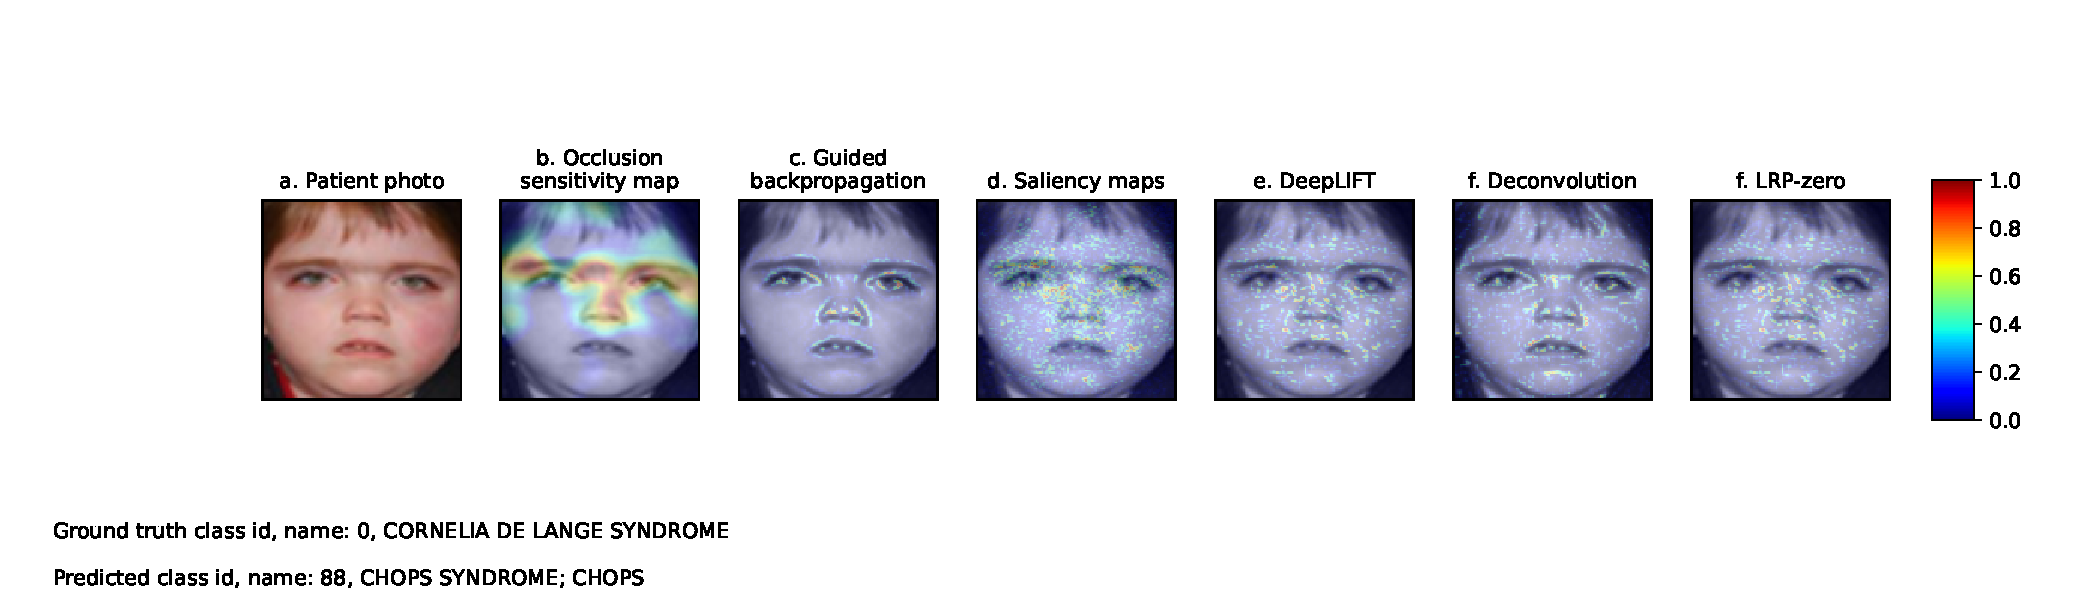
\includegraphics[width=1.02\textwidth, trim = 1cm 2.50cm 1cm 2.50cm, clip]{chapter4/1_2020.pdf}
    \end{figure}
    \section{Design of Experiments}
    \subsection{Overview}
    \subsection{Objectives}
    
    \section{Evaluation}
    \subsection{XAI Metrics}
    \subsection{Proposed Evaluation Strategy}
\end{document}
